\documentclass[aspectratio=43]{beamer}

% Title --------------------------------------------
\title{\huge Terrorism}
\author{Francisco Villamil}
\date{War, peace, and political violence\\UC3M, Fall 2023}

%%% NOTE -- CHECK THIS: https://github.com/paulgp/beamer-tips


%%% Building heavily on https://github.com/kylebutts/templates

% xcolor, define them
\usepackage{xcolor}

% TEXT COLORS
\definecolor{red}{HTML}{9a2515}
\definecolor{yellow}{HTML}{EBC944}
\definecolor{asher}{HTML}{555F61}
\definecolor{jet}{HTML}{131516}

% THEME COLORS
\definecolor{accent}{HTML}{107895}
\definecolor{accent2}{HTML}{9a2515}

% Color commands
\newcommand\red[1]{{\color{red}#1}}
\newcommand\yellow[1]{{\color{yellow}#1}}
\newcommand\asher[1]{{\color{asher}#1}}

\newcommand\BGred[1]{{\colorbox{red!80!white}{#1}}}
\newcommand\BGyellow[1]{{\colorbox{yellow!80!white}{#1}}}
\newcommand\BGasher[1]{{\colorbox{asher!80!white}{#1}}}

\renewcommand<>{\BGyellow}[1]{\only#2{\beameroriginal{\BGyellow}}{#1}}

% Appendix numbering
\usepackage{appendixnumberbeamer}

% Beamer Options -------------------------------------

% Background
\setbeamercolor{background canvas}{bg = white}

% Change text margins
\setbeamersize{text margin left = 25pt, text margin right = 15pt}

% \alert
\setbeamercolor{alerted text}{fg = accent2}

% Frame title
\setbeamercolor{frametitle}{bg = white, fg = jet}
\setbeamercolor{framesubtitle}{bg = white, fg = accent}
\setbeamerfont{framesubtitle}{size = \small, shape = \itshape}

% Block
\setbeamercolor{block title}{fg = white, bg = accent2}
\setbeamercolor{block body}{fg = jet, bg = jet!10!white}

% Title page
\setbeamercolor{title}{fg = jet}
\setbeamercolor{subtitle}{fg = accent}

%% Custom \maketitle and \titlepage
\setbeamertemplate{title page}
{
    \begin{centering}
      % \vspace{20mm}
      {\Large \usebeamerfont{title}\usebeamercolor[fg]{title}\inserttitle}\\ \vskip0.25em%
      \ifx\insertsubtitle\@empty%
      \else%
        {\usebeamerfont{subtitle}\usebeamercolor[fg]{subtitle}\insertsubtitle\par}%
      \fi%
      {\vspace{10mm}\insertauthor}\\
      \ifx\insertinstitute\@empty%
      \else%
        {\vspace{5mm}\color{asher}\scriptsize{\insertinstitute}}
      \fi%
      {\color{asher}\small{\insertdate}}\\
    \end{centering}
}

% Table of Contents
\setbeamercolor{section in toc}{fg = accent!70!jet}
\setbeamercolor{subsection in toc}{fg = jet}

% Button
\setbeamercolor{button}{bg = accent}

% Remove navigation symbols
\setbeamertemplate{navigation symbols}{}

% Table and Figure captions
\setbeamercolor{caption}{fg=jet!70!white}
\setbeamercolor{caption name}{fg=jet}
\setbeamerfont{caption name}{shape = \itshape}

% Put slide number / total slides at the bottom right
\makeatother
\makeatletter
\setbeamertemplate{footline} %{\hfill\insertframenumber/\inserttotalframenumber}
{%
  \leavevmode%
  \hbox{
  \begin{beamercolorbox}[wd=\paperwidth,ht=2.5ex,dp=1.125ex,leftskip=.3cm,rightskip=.3cm plus1fil]{footlinecolor}%
    \color{asher}{\hfill\insertframenumber/\inserttotalframenumber}
  \end{beamercolorbox}}%
  \vskip0pt%
}
\makeatother
\makeatletter

% Bullet points

%% Fix left-margins
\settowidth{\leftmargini}{\usebeamertemplate{itemize item}}
\addtolength{\leftmargini}{\labelsep}

%% enumerate item color
\setbeamercolor{enumerate item}{fg = accent}
\setbeamerfont{enumerate item}{size = \small}
\setbeamertemplate{enumerate item}{\insertenumlabel.}

%% itemize
\setbeamercolor{itemize item}{fg = accent!70!white}
\setbeamerfont{itemize item}{size = \small}
\setbeamertemplate{itemize item}[circle]
\setlength{\itemsep}{0pt plus 6pt}

%% right arrow for subitems
\setbeamercolor{itemize subitem}{fg = accent!60!white}
\setbeamerfont{itemize subitem}{size = \small}
\setbeamertemplate{itemize subitem}{$\rightarrow$}

\setbeamertemplate{itemize subsubitem}[square]
\setbeamercolor{itemize subsubitem}{fg = jet}
\setbeamerfont{itemize subsubitem}{size = \small}

% References

%% Bibliography Font, roughly matching aea
\setbeamerfont{bibliography item}{size = \footnotesize}
\setbeamerfont{bibliography entry author}{size = \footnotesize, series = \bfseries}
\setbeamerfont{bibliography entry title}{size = \footnotesize}
\setbeamerfont{bibliography entry location}{size = \footnotesize, shape = \itshape}
\setbeamerfont{bibliography entry note}{size = \footnotesize}

\setbeamercolor{bibliography item}{fg = jet}
\setbeamercolor{bibliography entry author}{fg = accent!60!jet}
\setbeamercolor{bibliography entry title}{fg = jet}
\setbeamercolor{bibliography entry location}{fg = jet}
\setbeamercolor{bibliography entry note}{fg = jet}

%% Remove bibliography symbol in slides
\setbeamertemplate{bibliography item}{}





% Links ----------------------------------------------

\usepackage{hyperref}
\hypersetup{
  colorlinks = true,
  linkcolor = accent,
  filecolor = accent,
  urlcolor = accent,
  citecolor = accent,
}


% Line spacing --------------------------------------
\usepackage{setspace}
\setstretch{1.2}


% \begin{columns} -----------------------------------
\usepackage{multicol}


% % Fonts ---------------------------------------------
% % Beamer Option to use custom fonts
% \usefonttheme{professionalfonts}
%
% % \usepackage[utopia, smallerops, varg]{newtxmath}
% % \usepackage{utopia}
% \usepackage[sfdefault,light]{roboto}
%
% % Small adjustments to text kerning
% \usepackage{microtype}



% Remove annoying over-full box warnings -----------
\vfuzz2pt
\hfuzz2pt


% Table of Contents with Sections
\setbeamerfont{myTOC}{series=\bfseries, size=\Large}
\AtBeginSection[]{
        \frame{
            \frametitle{Roadmap}
            \tableofcontents[current]
        }
    }


% References ----------------------------------------
\usepackage[
    citestyle= authoryear,
    style = authoryear,
    natbib = true,
    backend = biber
]{biblatex}

% Smaller font-size for references
\renewcommand*{\bibfont}{\small}

% Remove "In:"
\renewbibmacro{in:}{}

% Color citations for slides
\newenvironment{citecolor}
    {\footnotesize\begin{color}{accent2}}
    {\end{color}}

\newcommand{\citetcolor}[1]{{\footnotesize\textcolor{asher}{\citet{#1}}}}
\newcommand{\citepcolor}[1]{{\footnotesize\textcolor{asher}{\citep{#1}}}}

% Tables -------------------------------------------
% Tables too big
% \begin{adjustbox}{width = 1.2\textwidth, center}
\usepackage{adjustbox}
\usepackage{array}
\usepackage{threeparttable, booktabs, adjustbox}

% Fix \input with tables
% \input fails when \\ is at end of external .tex file

\makeatletter
\let\input\@@input
\makeatother

% Tables too narrow
% \begin{tabularx}{\linewidth}{cols}
% col-types: X - center, L - left, R -right
% Relative scale: >{\hsize=.8\hsize}X/L/R
\usepackage{tabularx}
\newcolumntype{L}{>{\raggedright\arraybackslash}X}
\newcolumntype{R}{>{\raggedleft\arraybackslash}X}
\newcolumntype{C}{>{\centering\arraybackslash}X}

% Figures

% \imageframe{img_name} -----------------------------
% from https://github.com/mattjetwell/cousteau
\newcommand{\imageframe}[1]{%
    \begin{frame}[plain]
        \begin{tikzpicture}[remember picture, overlay]
            \node[at = (current page.center), xshift = 0cm] (cover) {%
                \includegraphics[keepaspectratio, width=\paperwidth, height=\paperheight]{#1}
            };
        \end{tikzpicture}
    \end{frame}%
}

% subfigures
\usepackage{subfigure}


% Highlight slide -----------------------------------
% \begin{transitionframe} Text \end{transitionframe}
% from paulgp's beamer tips
\newenvironment{transitionframe}{
    \setbeamercolor{background canvas}{bg=accent!60!black}
    \begin{frame}\color{accent!10!white}\LARGE\centering
}{
    \end{frame}
}


% Table Highlighting --------------------------------
% Create top-left and bottom-right markets in tabular cells with a unique matching id and these commands will outline those cells
\usepackage[beamer,customcolors]{hf-tikz}
\usetikzlibrary{calc}
\usetikzlibrary{fit,shapes.misc}

% To set the hypothesis highlighting boxes red.
\newcommand\marktopleft[1]{%
    \tikz[overlay,remember picture]
        \node (marker-#1-a) at (0,1.5ex) {};%
}
\newcommand\markbottomright[1]{%
    \tikz[overlay,remember picture]
        \node (marker-#1-b) at (0,0) {};%
    \tikz[accent!80!jet, ultra thick, overlay, remember picture, inner sep=4pt]
        \node[draw, rectangle, fit=(marker-#1-a.center) (marker-#1-b.center)] {};%
}



\begin{document}

\begin{frame}
  \titlepage
\end{frame}

% ----------------------------------------------------
\begin{frame}
\frametitle{}
\centering

\begin{itemize}
  \item What is terrorism?
\end{itemize}

\end{frame}
% ----------------------------------------------------

% ----------------------------------------------------
\imageframe{img/9-11}
% ----------------------------------------------------

% ----------------------------------------------------
\imageframe{img/obama-war-on-terror}
% ----------------------------------------------------

% ----------------------------------------------------
\begin{frame}
\frametitle{What is terrorism?}
\centering

\visible<2->{
\begin{itemize}
  \item Violence against civilians?
\end{itemize}
}

\vspace{20pt}

\visible<3>{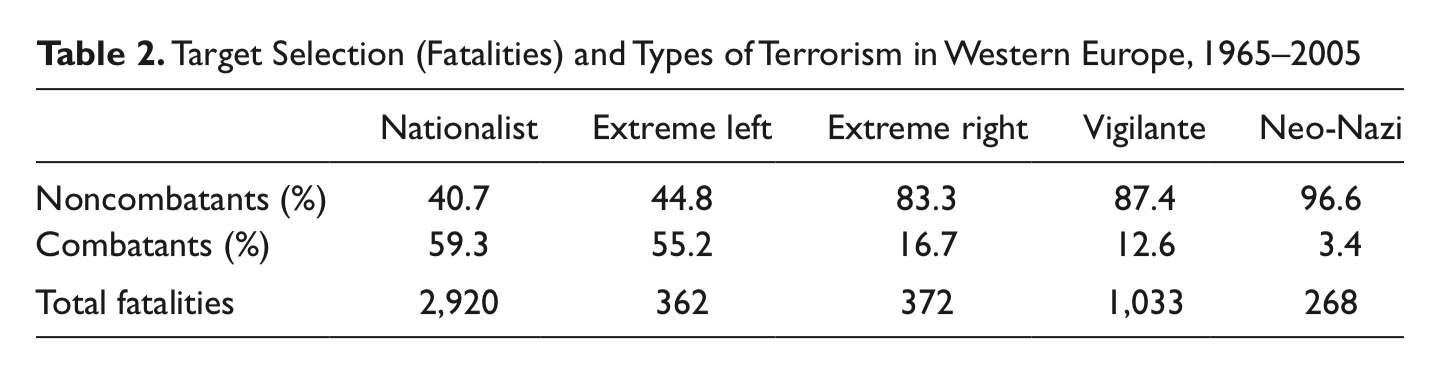
\includegraphics[width = \textwidth]{img/combatants-noncombatant}}

\end{frame}
% ----------------------------------------------------

% ----------------------------------------------------
\begin{frame}
\frametitle{What is terrorism?}
\centering

\begin{itemize}
  \item `Communicative' violence?
\end{itemize}

\vspace{20pt}

\visible<2>{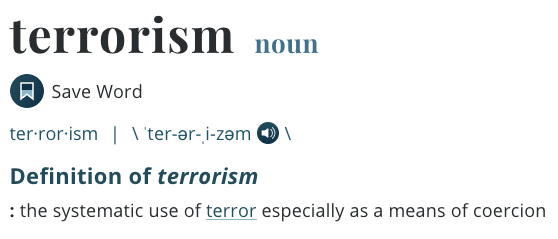
\includegraphics[width = 0.7\textwidth]{img/webster}}

\end{frame}
% ----------------------------------------------------

% ----------------------------------------------------
\imageframe{img/wikipedia}
% ----------------------------------------------------

% ----------------------------------------------------
\imageframe{img/represion-franquista}
% ----------------------------------------------------

% ----------------------------------------------------
\begin{frame}
\frametitle{}
\centering

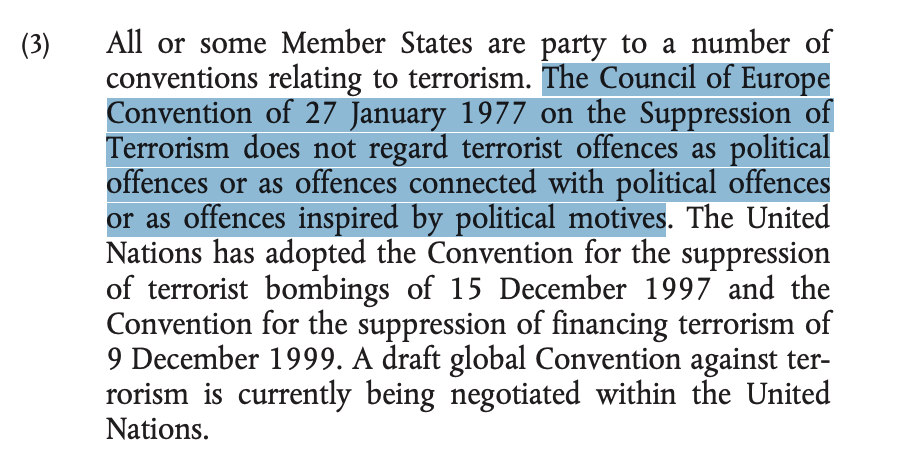
\includegraphics[width = 0.9\textwidth]{img/eu_law}

EU Framework Decision on Terrorism, 2002

\end{frame}
% ----------------------------------------------------

% ----------------------------------------------------
\begin{frame}
\frametitle{Understanding terrorism}
\centering

\begin{itemize}
  \item[] This is not very useful for understanding anything at all
  \begin{itemize}
    \item<2-> Identifying terrorism?
    \item<3-> \red{Political} incentives for the use of terrorism?
    \item<4-> {\color{red}{Who}} and {\color{red}{when}} uses it?
    \item<5-> What does \textbf{prevention} mean? And how do we do it?
  \end{itemize}
\end{itemize}

\end{frame}
% ----------------------------------------------------

% ----------------------------------------------------
\begin{frame}
\frametitle{Understanding terrorism}
\centering

\begin{itemize}
  \item[] There are two ways to look at this
  \item[]
  \item<2-> \BGyellow{Terrorism}: the action
  \visible<3->{\begin{itemize}
    \item What is a terrorist attack?
    \item How is it different from other forms of political violence?
    \item Why do actors choose terrorism over other forms of violence?
  \end{itemize}}
  \item<2-> \BGyellow{Terrorists}: the actor
  \visible<4->{\begin{itemize}
    \item Why do actors rely \textbf{primarily} on terrorism?
    \item Important: What is the `opposite' of terrorism?
  \end{itemize}}
\end{itemize}

\end{frame}
% ----------------------------------------------------

% ----------------------------------------------------
\begin{frame}[plain]

    \begin{tikzpicture}[remember picture, overlay]
        \node[at = (current page.center), xshift = 0cm, yshift = 1cm] (cover) {%
            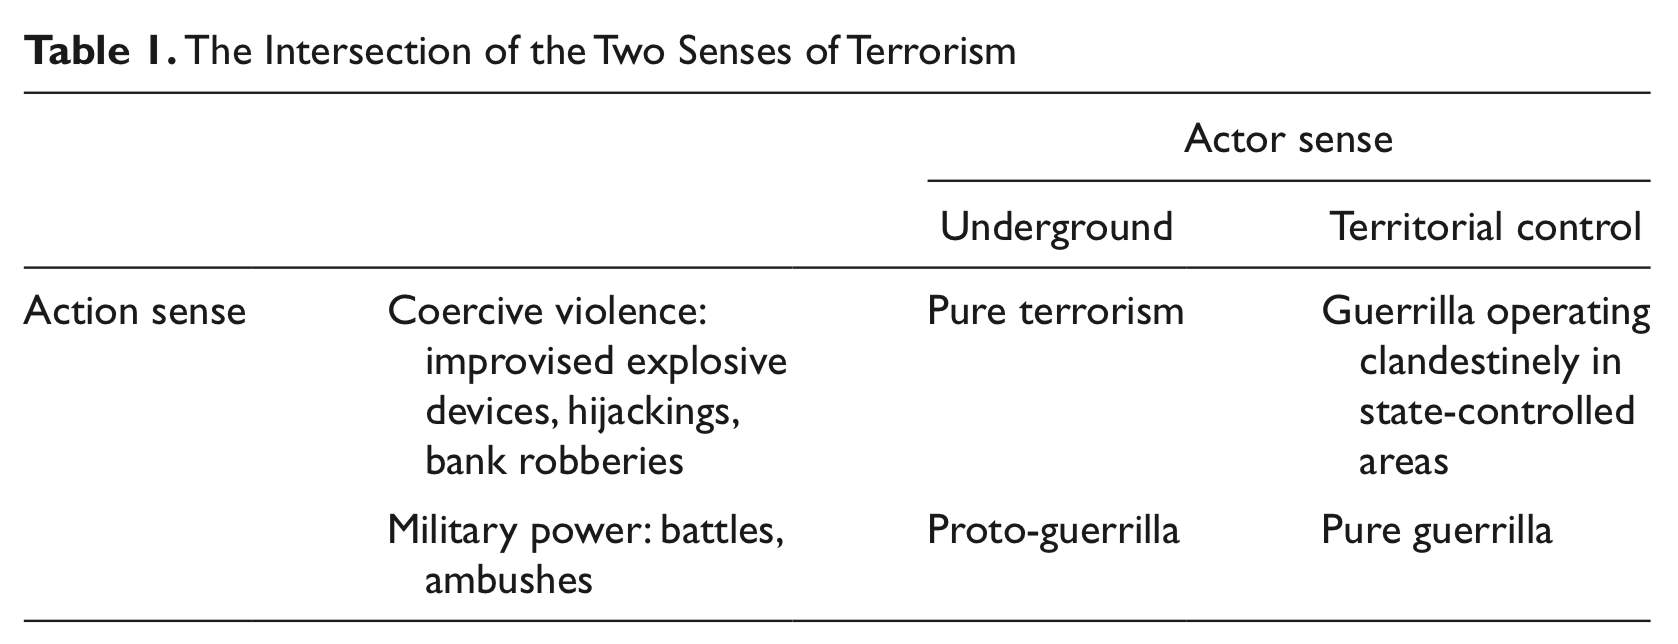
\includegraphics[keepaspectratio, width=\paperwidth, height=\paperheight]{img/actor-action-sense}
        };
    \end{tikzpicture}

    \vspace{200pt}

    \asher{{\scriptsize De la Calle \& Sánchez-Cuenca (2011) What we talk about when we talk about terrorism. \textit{Politics \& Society} 39(3): 451--472.\\}}

\end{frame}
% ----------------------------------------------------

% ----------------------------------------------------
\begin{frame}[plain]

    \begin{tikzpicture}[remember picture, overlay]
        \node[at = (current page.center), xshift = 0cm, yshift = 1cm] (cover) {%
            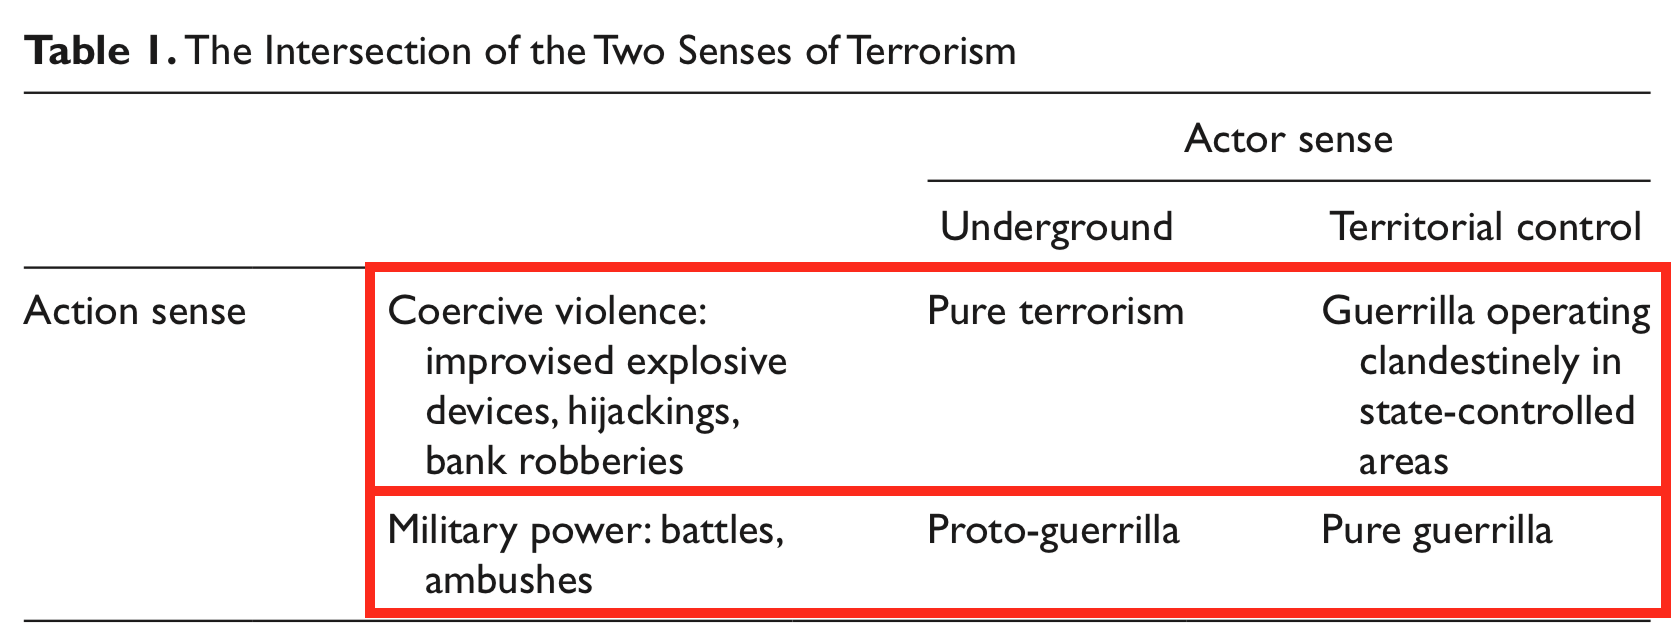
\includegraphics[keepaspectratio, width=\paperwidth, height=\paperheight]{img/actor-action-sense1}
        };
    \end{tikzpicture}

    \vspace{160pt}

    \begin{itemize}
      \item Terrorism as an \BGyellow{action}: military power vs the power to hurt
      \item Coercive nature of terrorist violent, compatible with having low military capacity
    \end{itemize}

\end{frame}
% ----------------------------------------------------

% ----------------------------------------------------
\begin{frame}[plain]

    \begin{tikzpicture}[remember picture, overlay]
        \node[at = (current page.center), xshift = 0cm, yshift = 1cm] (cover) {%
            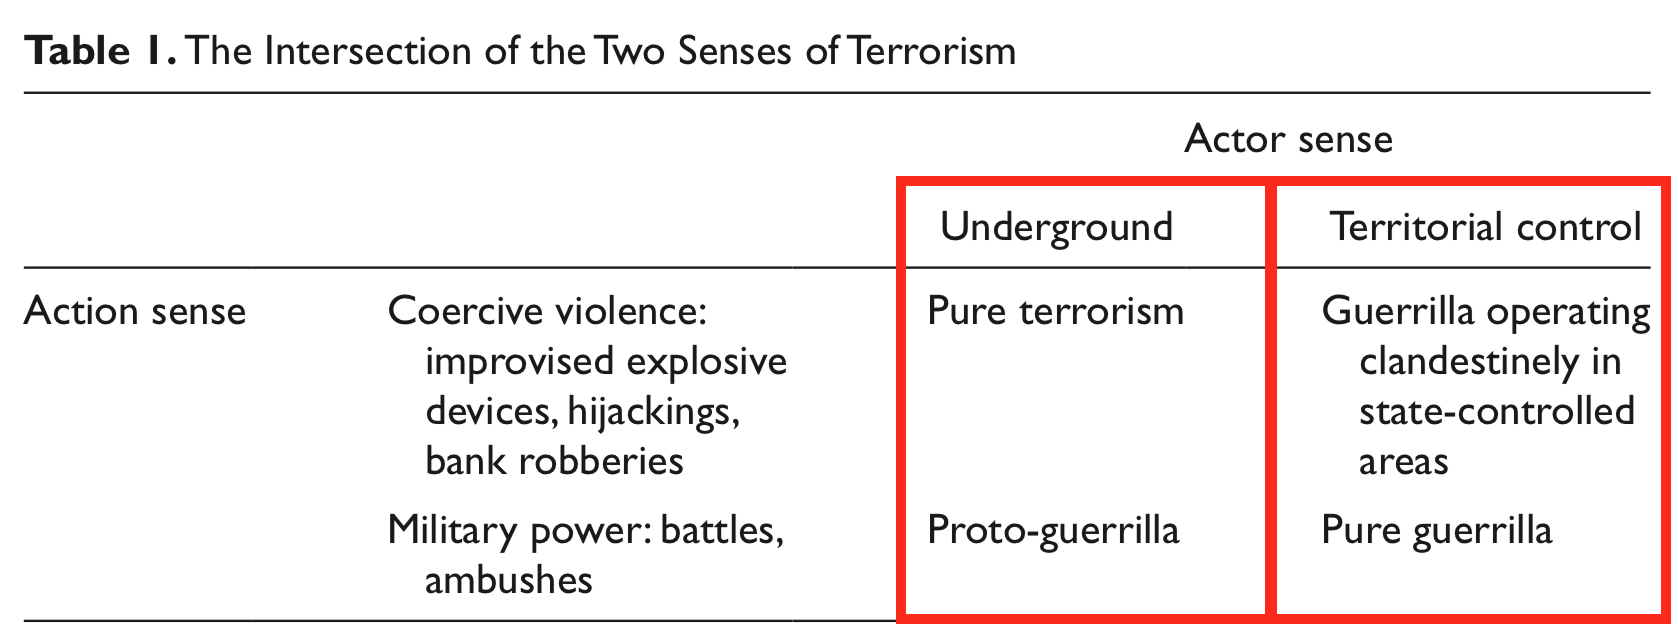
\includegraphics[keepaspectratio, width=\paperwidth, height=\paperheight]{img/actor-action-sense2}
        };
    \end{tikzpicture}

    \vspace{150pt}

    \begin{itemize}
      \item Terrorists as \BGyellow{actors}: underground groups without territory
      \item \textit{Duopoly} of violence (vs fragmented monopoly)
    \end{itemize}

\end{frame}
% ----------------------------------------------------

% ----------------------------------------------------
\begin{frame}[plain]

    \begin{tikzpicture}[remember picture, overlay]
        \node[at = (current page.center), xshift = 0cm, yshift = 1cm] (cover) {%
            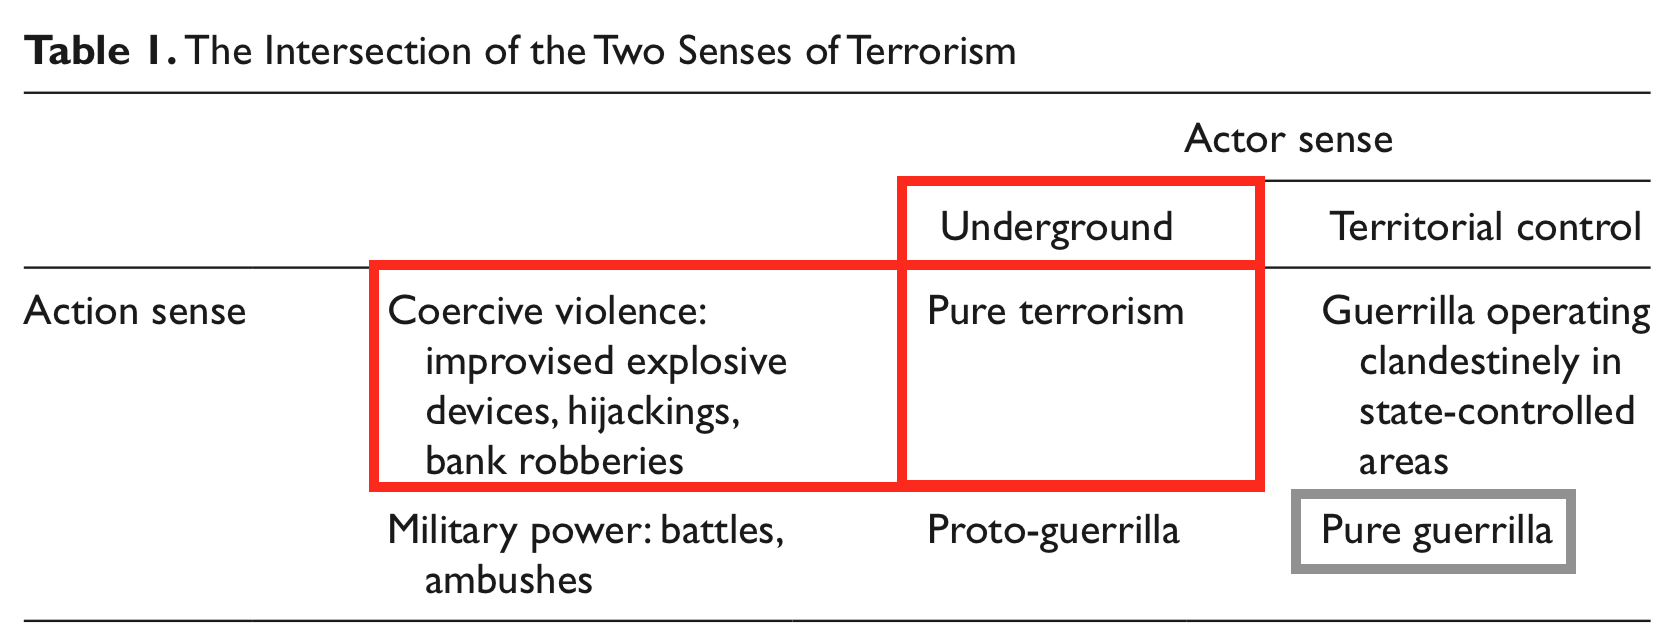
\includegraphics[keepaspectratio, width=\paperwidth, height=\paperheight]{img/actor-action-sense3}
        };
    \end{tikzpicture}

    \vspace{160pt}

    \begin{itemize}
      \item {\color{red}{`Pure terrorism'}}: underground groups that use coercive violence because they don't have any military capacity
      \item<2-> It's easy to distinguish between ideal types (guerrillas and terrorists)
    \end{itemize}

\end{frame}
% ----------------------------------------------------

% ----------------------------------------------------
\imageframe{img/eta-mesa}
% ----------------------------------------------------

% ----------------------------------------------------
\imageframe{img/farc}
% ----------------------------------------------------

% ----------------------------------------------------
\begin{frame}[plain]

    \begin{tikzpicture}[remember picture, overlay]
        \node[at = (current page.center), xshift = 0cm, yshift = 1cm] (cover) {%
            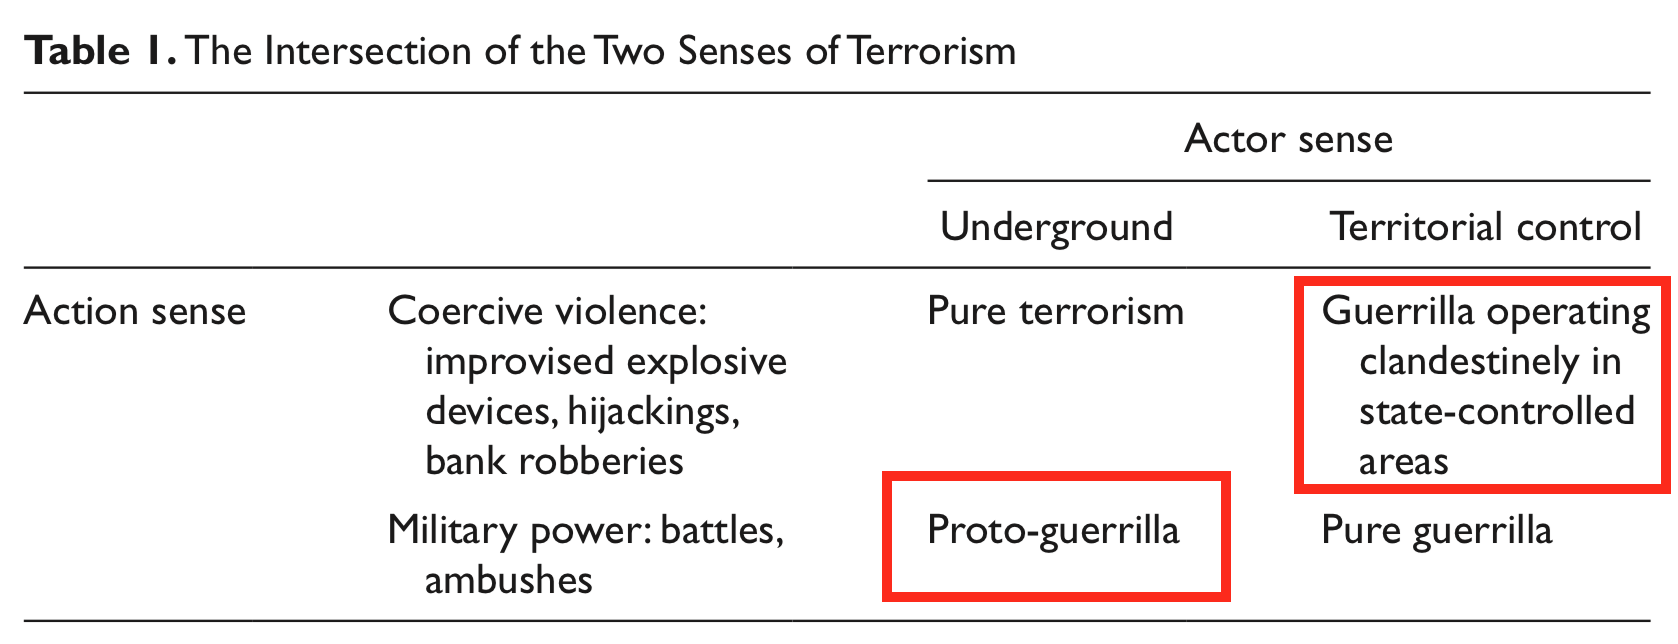
\includegraphics[keepaspectratio, width=\paperwidth, height=\paperheight]{img/actor-action-sense4}
        };
    \end{tikzpicture}

    \vspace{150pt}

    \begin{itemize}
      \item But there are also `hybrid' types, especially groups that control territory \textit{and} employ terrorist violence (urban guerrilla is way less common)
      % \item Many examples: Shinning Path in Peru, PKK in Turkey, etc
      % \item (Urban guerrilla is way less common: Tupamaros in Uruguay, Monteneros in Argentina, ...)
    \end{itemize}

\end{frame}
% ----------------------------------------------------

% ----------------------------------------------------
\imageframe{img/montoneros}
% ----------------------------------------------------

% ----------------------------------------------------
\begin{frame}
\frametitle{More on hybrid types}
\centering

\begin{itemize}
  \item It's not only about groups that always remain the same, some of them {\color{red}{transition over time}}
  \begin{itemize}
    \item<2-> From guerrilla to underground groups: PKK in the late 1990s
    \item<3-> From underground to guerrilla: Hezbollah after 1990
  \end{itemize}
\end{itemize}


\end{frame}
% ----------------------------------------------------

% ----------------------------------------------------
\imageframe{img/hezbollah}
% ----------------------------------------------------

% ----------------------------------------------------
\imageframe{img/south_armagh}
% ----------------------------------------------------

% ----------------------------------------------------
\begin{frame}
\frametitle{More on hybrid types}
\centering

\begin{itemize}
  \item And there is also variation in {\color{red}{space}}
  \begin{itemize}
    \item<2-> A group might use guerrilla methods in one area but terrorist actions in another part of the country
    \item<3-> Actions constrained by military capacities
  \end{itemize}
\end{itemize}



\end{frame}
% ----------------------------------------------------

% ----------------------------------------------------
\begin{frame}
\frametitle{Variation across space \& time: Shinning Path}
\centering

\begin{minipage}{0.49\textwidth}\centering
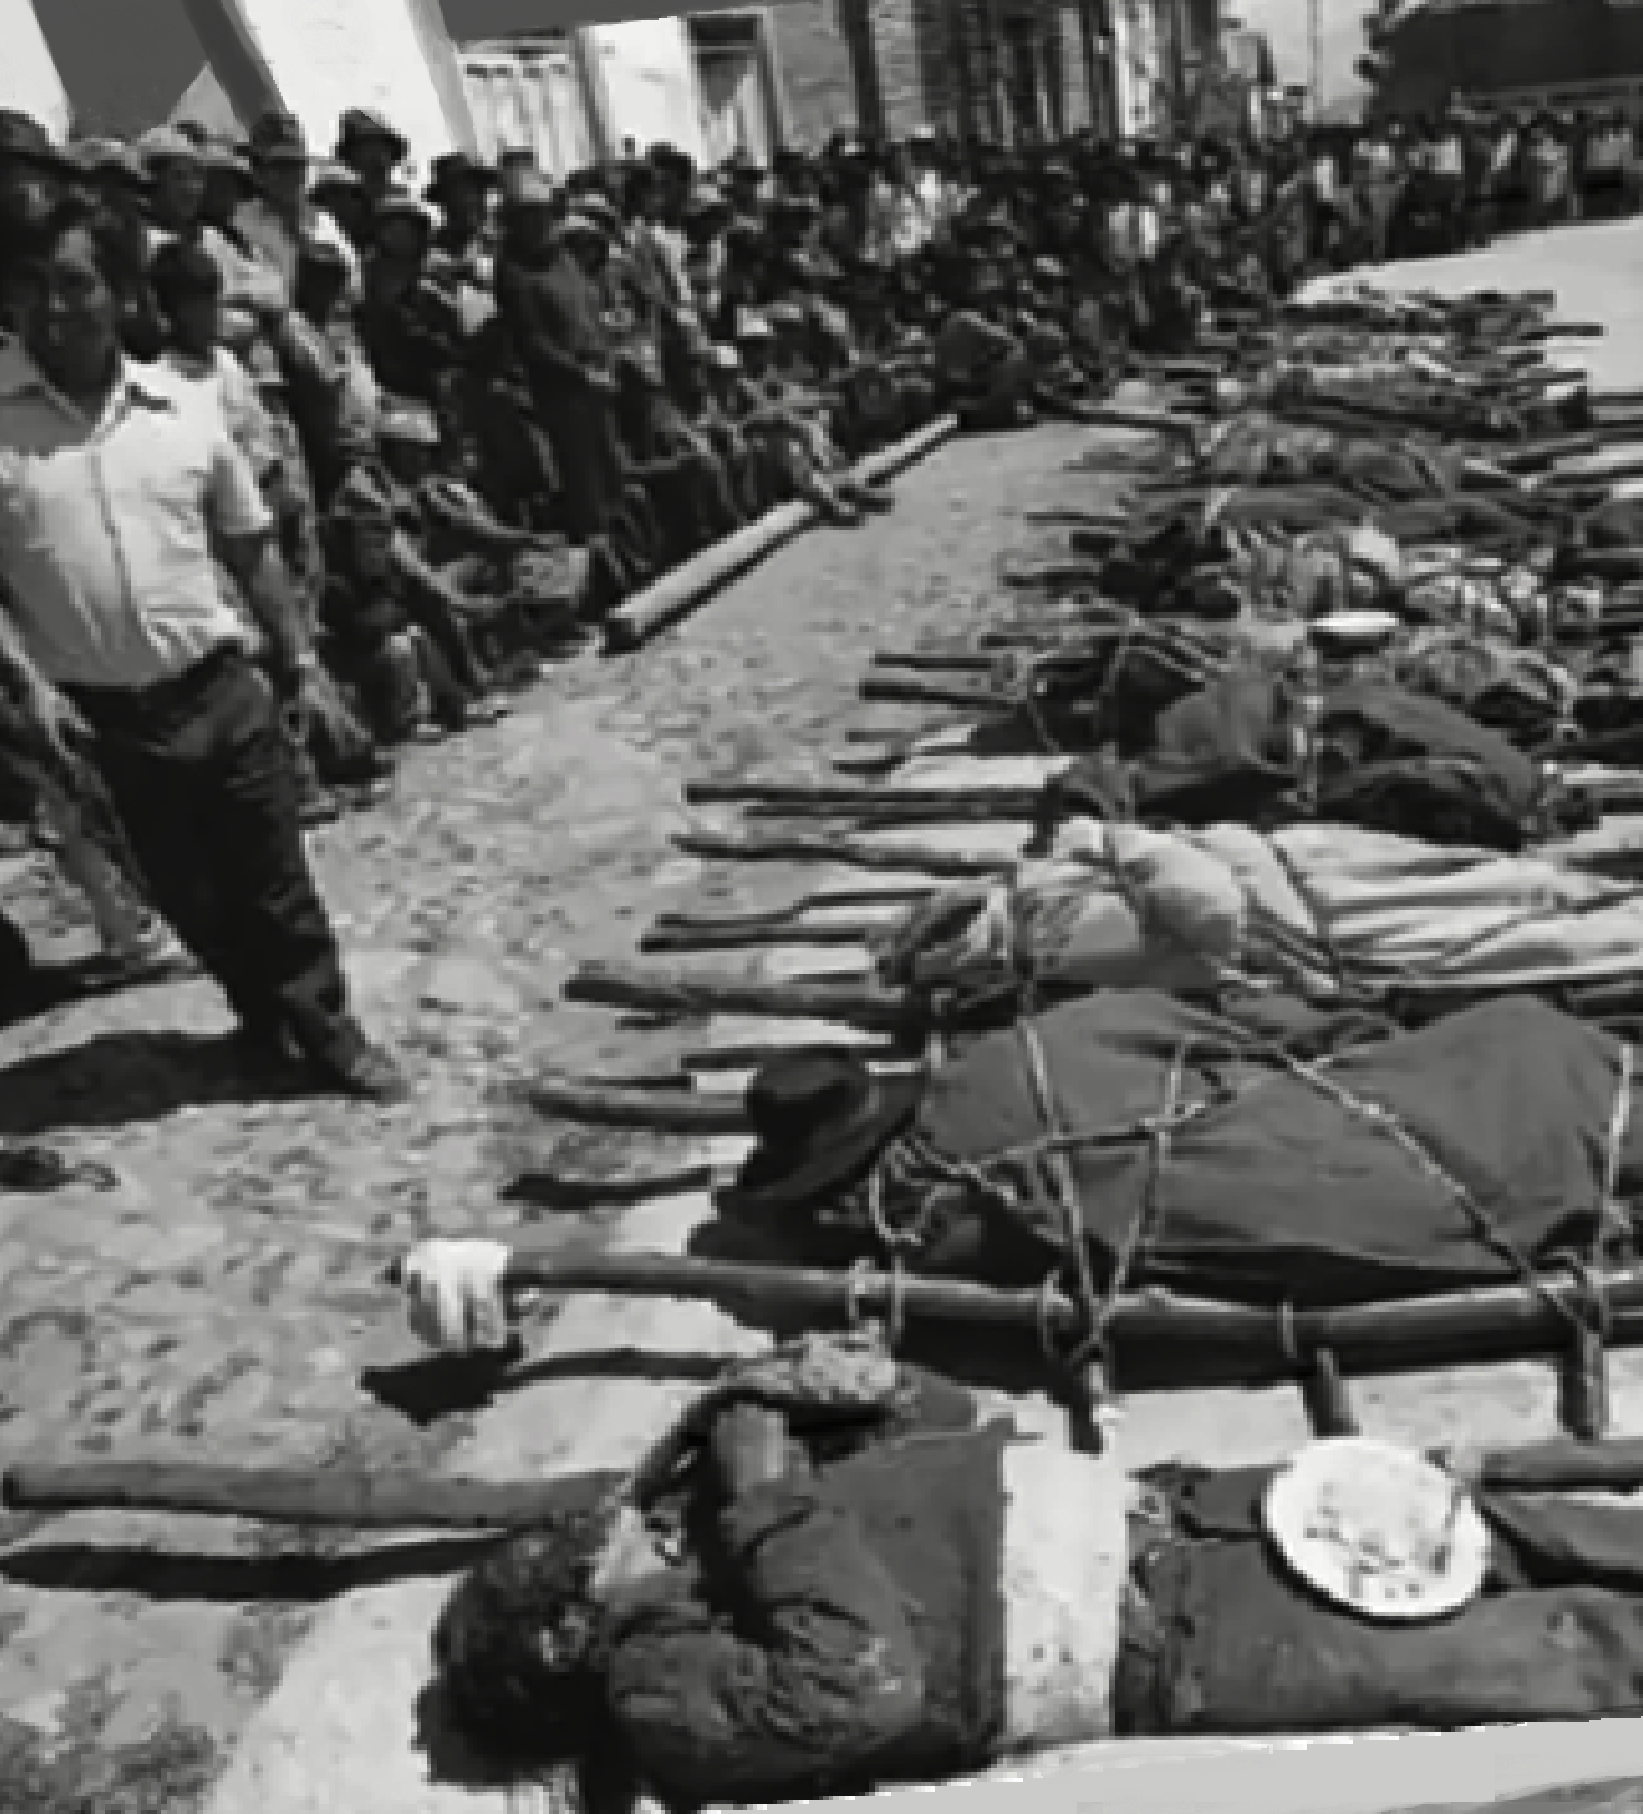
\includegraphics[width = 0.9\textwidth]{img/lucanamarca}\\
{\small Lucanamarca Massacre\\(Sendero Luminoso, 1983)}\\
\end{minipage}\hfill
\visible<2>{\begin{minipage}{0.49\textwidth}\centering
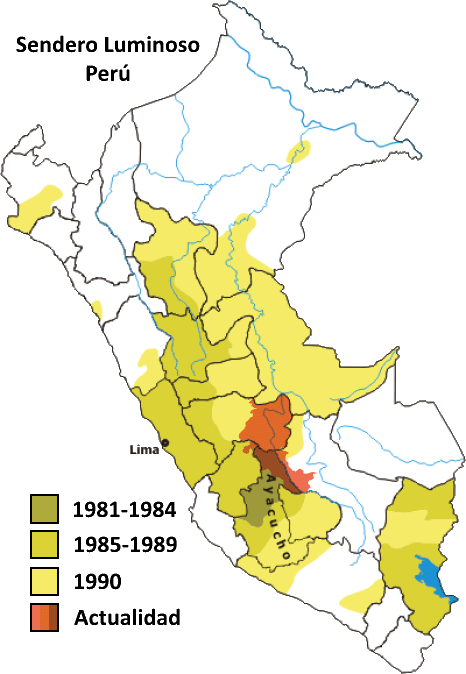
\includegraphics[width = 0.6\textwidth]{img/lucanamarca-peru-map}\\
\begin{itemize}
  \item Massacre in response to local opposition
  \item Area controlled by SL
\end{itemize}
\end{minipage}}

\end{frame}
% ----------------------------------------------------

% ----------------------------------------------------
\begin{frame}
\frametitle{Variation across space \& time: Shinning Path}
\centering

\begin{minipage}{0.59\textwidth}\centering
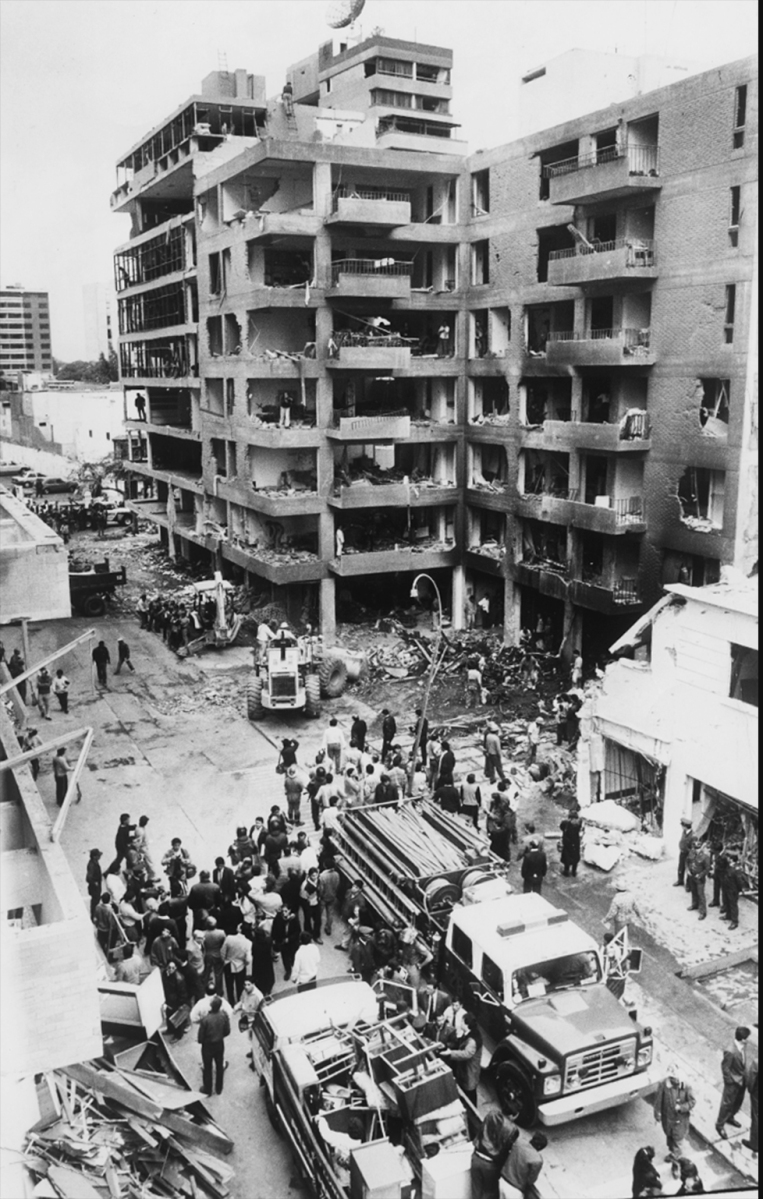
\includegraphics[width = 0.7\textwidth]{img/tarata}\\
{\small Calle Tarata bombing (Summer 1992)}\\
\end{minipage}\hfill
\visible<2>{\begin{minipage}{0.39\textwidth}\centering
\begin{itemize}
  \item Context of declining power by SL
  \begin{itemize}
    \item Fujimori's \textit{autogolpe}
  \end{itemize}
  \item Switch in SL tactics, different place
\end{itemize}
\end{minipage}}

\end{frame}
% ----------------------------------------------------

% ----------------------------------------------------
\begin{frame}
\frametitle{Understanding the \textit{emergence} of terrorism}
\centering

\begin{itemize}
  \item So how does this help in practice?
\end{itemize}


\end{frame}
% ----------------------------------------------------

% ----------------------------------------------------
\begin{frame}
\frametitle{Understanding the \textit{emergence} of terrorism}
\centering

\begin{itemize}
  \item The relevant question usually focuses on the \textit{actor sense}:
  \item[] {\color{red}{\textbf{when does a domestic terrorist group emerge?}}}
  \begin{itemize}
    \item i.e., an underground group that relies almost exclusively on terrorist/coercive violence
  \end{itemize}
  \item<2-> Action-sense: covers too many different things
  \begin{itemize}
    \item when is it used?
    \item by whom?
    \item what shape does it take?
  \end{itemize}
\end{itemize}


\end{frame}
% ----------------------------------------------------

% ----------------------------------------------------
\begin{frame}
\frametitle{Understanding the \textit{emergence} of terrorism}
\centering

\begin{itemize}
  \item[1.] \BGyellow<1>{{\color{red}{State capacity}}}
  \begin{itemize}
    \item Remember civil war onset and state capacity
    \item Terrorists are the guerrillas of richer countries
  \end{itemize}
  \item<2->[2.] \BGyellow<2>{{\color{red}{Regime type}}}
  \begin{itemize}
    \item U-type relationship between repressive/democratic regimes and the onset of terrorism
  \end{itemize}
  \item<3->[3.] \BGyellow<3>{{\color{red}{Historical path-dependence}}}
  \begin{itemize}
    \item Interwar Europe and terrorism after the 1960s/70s
    \item[] {\scriptsize (In countries with a non-liberal path, the Left was more radicalized, but in liberal countries, social [leftist] support for violence was much lower $\rightarrow$ armed groups restraint)}
  \end{itemize}
\end{itemize}


\end{frame}
% ----------------------------------------------------

% ----------------------------------------------------
\begin{frame}
\frametitle{Terrorists and the state}
\centering

\begin{itemize}
  \item What \textbf{do {\color{red}{states}} do to stop terrorism?}
  \item[]<2-> Does it work?
\end{itemize}

\end{frame}
% ----------------------------------------------------

% ----------------------------------------------------
\begin{frame}
\frametitle{Terrorists and the state}
\centering

\begin{itemize}
  \item[1.] {\color{red}{\textbf{State repression} (and counter-terrorist violence}})
  \item<2-> \textbf{Risk of backlash}: counterreaction to state violence
  \item[\textcolor{white}{\textbullet}] {\color{white} Indiscriminate or selective violence? The US and the COINTELPRO against the left and the Black Liberation Movement}
  \begin{itemize}\color{white}
    \item[\textcolor{white}{\textbullet}] Perhaps this is about state capacity and the quality of intelligence services: the killing of Melitón Manzanas in 1968 and subsequent mass detentions
  \end{itemize}
\end{itemize}

\end{frame}
% ----------------------------------------------------

% ----------------------------------------------------
\begin{frame}
\frametitle{Terrorists and the state}
\centering

\begin{itemize}
  \item Bloody Sunday (1972) in Northern Ireland
\end{itemize}

\vspace{10pt}

\begin{minipage}{0.49\textwidth}\centering
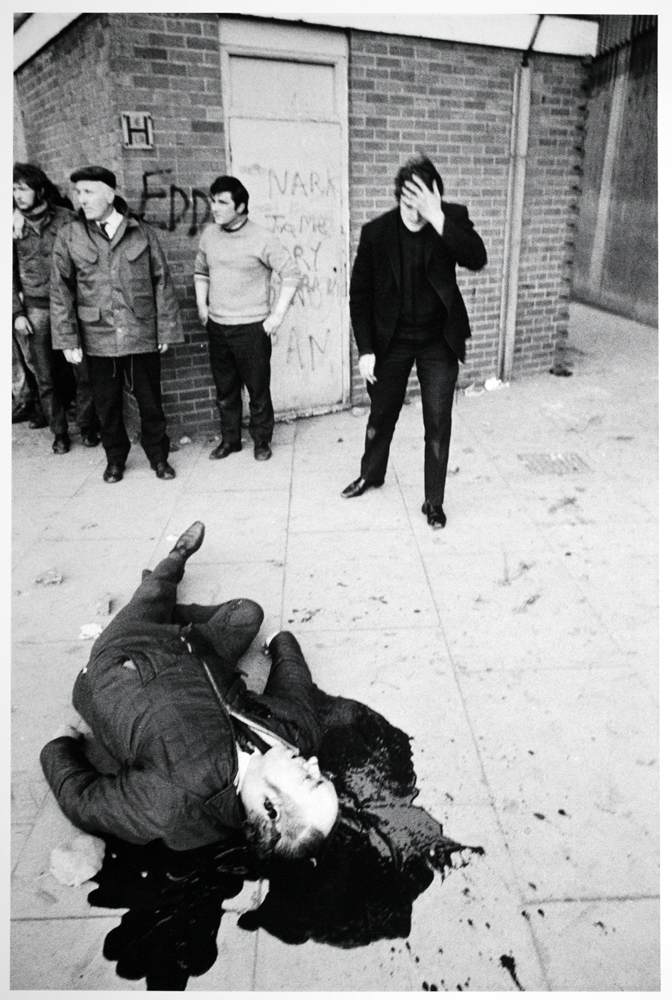
\includegraphics[width = 0.8\textwidth]{img/bloody-sunday}
\end{minipage}\hfill
\begin{minipage}{0.49\textwidth}\centering
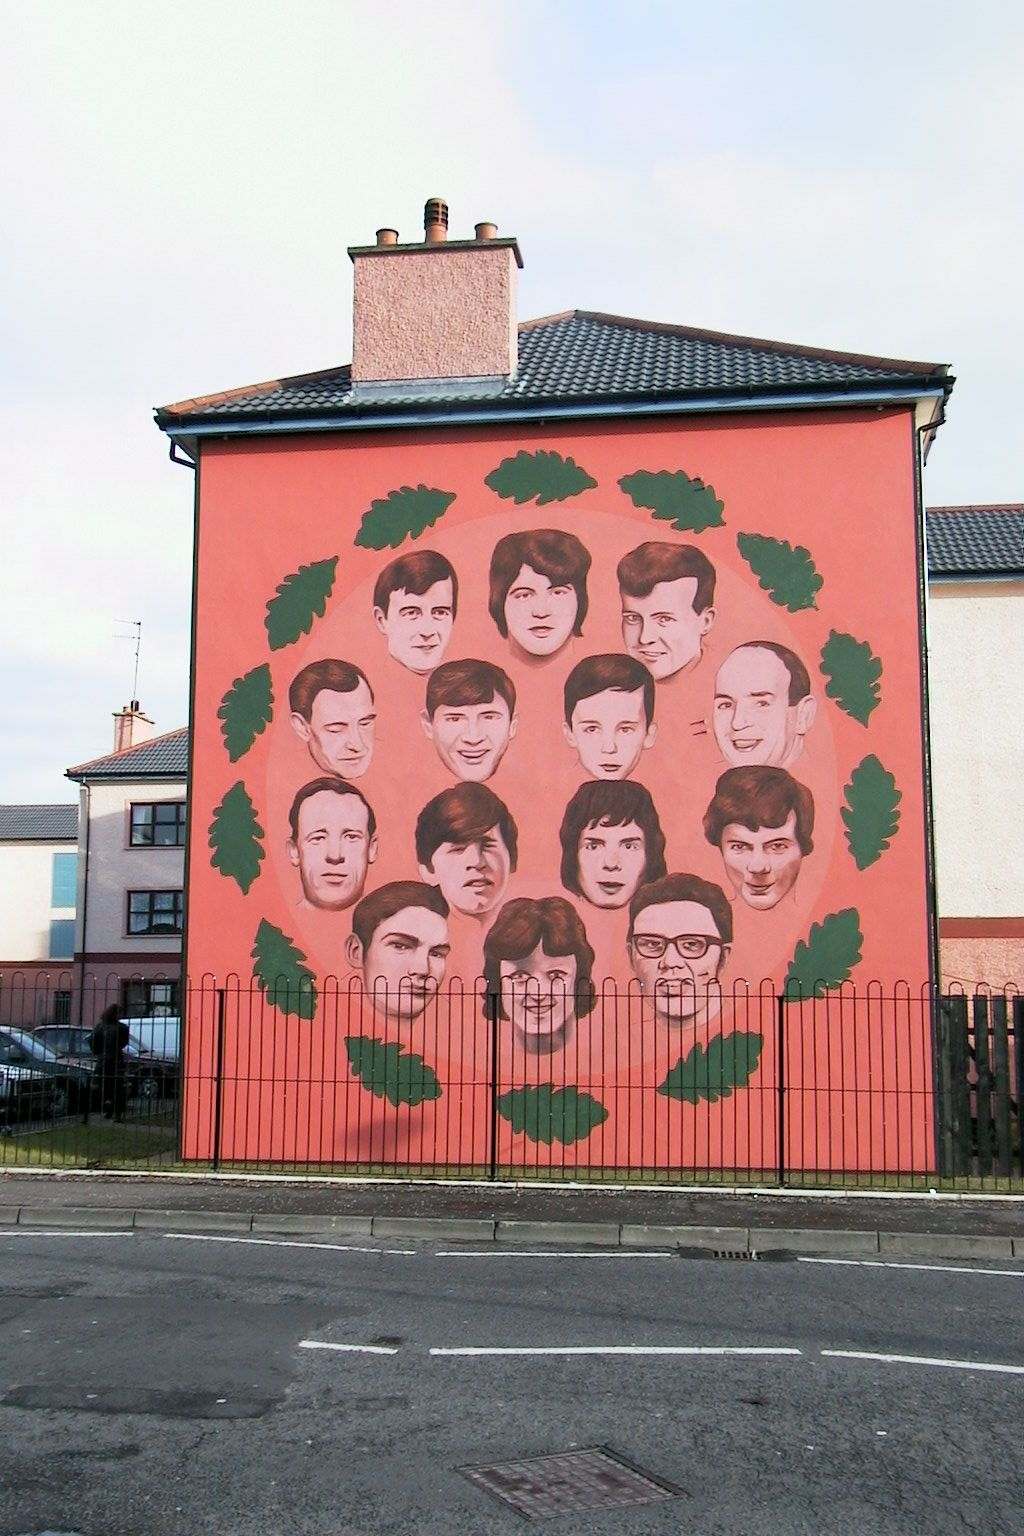
\includegraphics[width = 0.8\textwidth]{img/bloody-sunday-mural}
\end{minipage}

\end{frame}
% ----------------------------------------------------

% ----------------------------------------------------
\begin{frame}
\frametitle{Terrorists and the state}
\centering

\begin{itemize}
  \item[1.] State repression and counter-terrorist violence, {\color{red}{does it work?}}
  \item Risk of backlash effect: counterreaction to state violence
  \item \textbf{Indiscriminate or selective violence?} The US and the COINTELPRO against the Left and the Black Power movt
  \begin{itemize}
    \item<2-> Perhaps this is about state capacity and the quality of intelligence services: the killing by ETA of Melitón Manzanas in 1968 and subsequent mass detentions
  \end{itemize}
\end{itemize}

\end{frame}
% ----------------------------------------------------

% ----------------------------------------------------
\begin{frame}
\frametitle{Terrorists and the state}
\centering

\begin{itemize}
  \item[2.] {\color{red}{\textbf{Policy concessions}}}
  \item<2-> Timing is important: before or after terrorist group formation?
  \item<3-> Concessions could avoid the formation of terrorist groups, or deincentive the use of violence
  \item<4-> But it can also be counter-productive
  \begin{itemize}
    \item If group is not cohesive, \textit{spoiling} response by radicals
    \item Imitation dynamics for other groups?
  \end{itemize}
  \item<5-> Overall, no clear patterns
\end{itemize}

\end{frame}
% ----------------------------------------------------

% ----------------------------------------------------
\begin{frame}
\frametitle{Terrorists and society}
\centering

\begin{itemize}[<+->]
  \item What is the \textbf{relationship between {\color{red}{terrorists and civilians}}?}
  \item[] How do they manage it?
  \item[]<2-> {\color{white}{And how are they influenced by it?}}
\end{itemize}

\end{frame}
% ----------------------------------------------------

% ----------------------------------------------------
\begin{frame}
\frametitle{Terrorists and society}
\centering

\begin{itemize}[<+->]
  \item Terrorists \textit{and} guerrilla groups need some \textbf{social support} to survive, but not in the same way
  \item In common: both need to enforce cooperation and deincentive defection or betrayal
  \item But {\color{red}{\textbf{guerrillas}}} have more \textbf{local coercive power}, even in cases of fragmented sovereignty
  \item {\color{red}{\textbf{Terrorists}}} do not have that power, they act underground and usually in a context where the state is dominant (no need to choose sides)
\end{itemize}

\end{frame}
% ----------------------------------------------------

% ----------------------------------------------------
\begin{frame}
\frametitle{Terrorists and society}
\centering

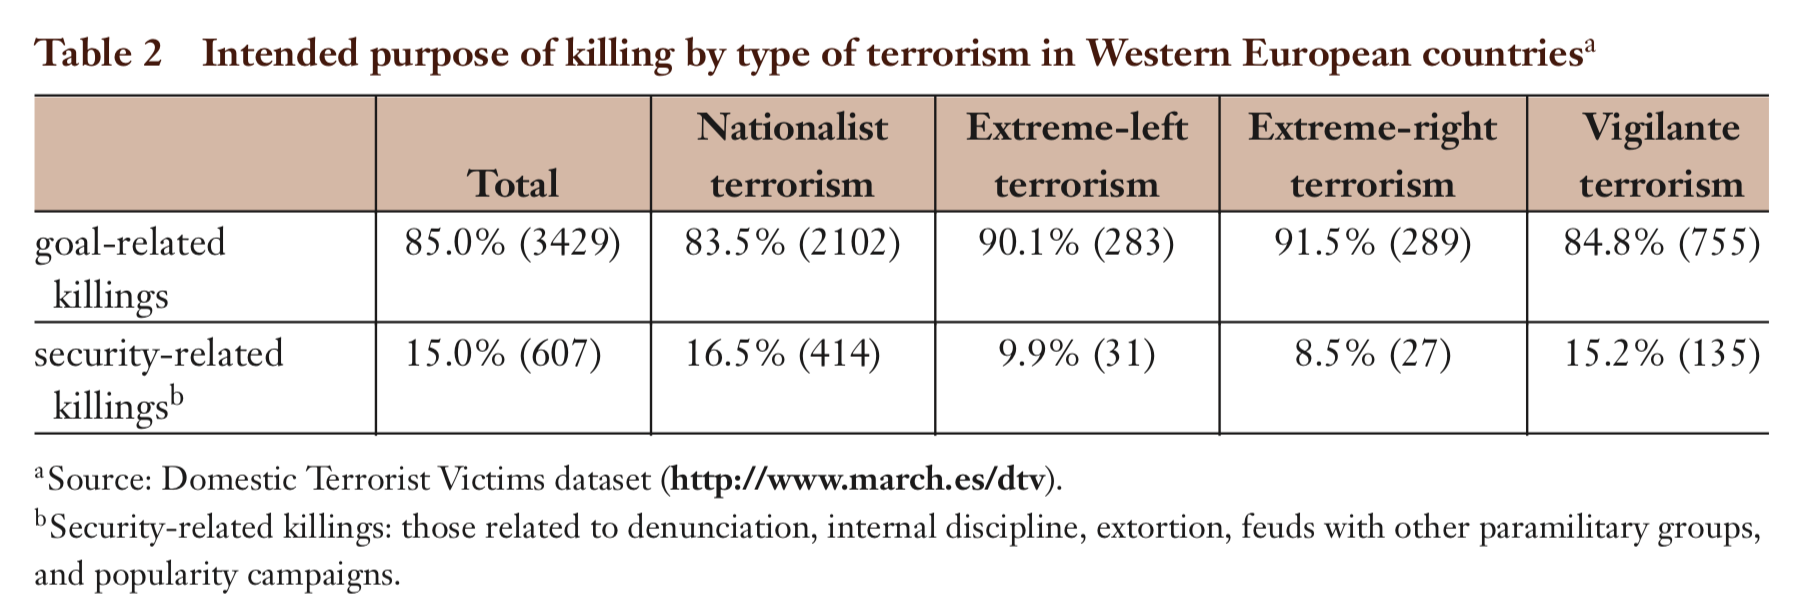
\includegraphics[width = \textwidth]{img/goal-security-killings}

\vspace{20pt}

\visible<2->{
\begin{itemize}
  \item Which explains why so many killings are security-related
  \begin{itemize}
    \item Differences between terrorist organizations: {\color{red}{nationalist and vigilante groups}} are more concerned with territory (and civilian constituencies)
  \end{itemize}
\end{itemize}
}

\end{frame}
% ----------------------------------------------------

% ----------------------------------------------------
\begin{frame}
\frametitle{Terrorists and society}
\centering

\begin{itemize}
  \item[] What is the \textbf{relationship between {\color{red}{terrorists and civilians}}?}
  \item[] How do they manage it?
  \item[]<2-> And how are they {\color{red}{influenced}} by it?
\end{itemize}

\end{frame}
% ----------------------------------------------------

% ----------------------------------------------------
\begin{frame}
\frametitle{Terrorists and society}
\centering

\begin{itemize}
  \visible{\item[1.] If \textbf{population is {\color{red}{more moderate}}}: trade-off between acceptance of violence by society, and the use of violence to advance political means
  \begin{itemize}
    \item Particularly in the case of indiscriminate violence
    \item `Extreme' people will likely think the same, but there is a risk of making moderates switch to the opposite side
    \item This constraint explains why terrorist groups restraint themselves
  \end{itemize}}
  \visible<2->{\item[2.] Opposite dynamics when the \textbf{population is {\color{red}{as radicalized as}}} the terrorists
  \begin{itemize}
    \item Competition among groups and outbidding processes
    \item Higher risk of escalation
  \end{itemize}}
\end{itemize}

\end{frame}
% ----------------------------------------------------

% ----------------------------------------------------
\begin{frame}
\frametitle{Terrorists and society}
\centering

\begin{itemize}
  \item[3.] Also, terrorist violence can be a {\color{red}{substitute}} or a reaction to declining levels of mobilization
\end{itemize}

\end{frame}
% ----------------------------------------------------

% ----------------------------------------------------
\begin{frame}
\frametitle{Terrorists and society}
\centering

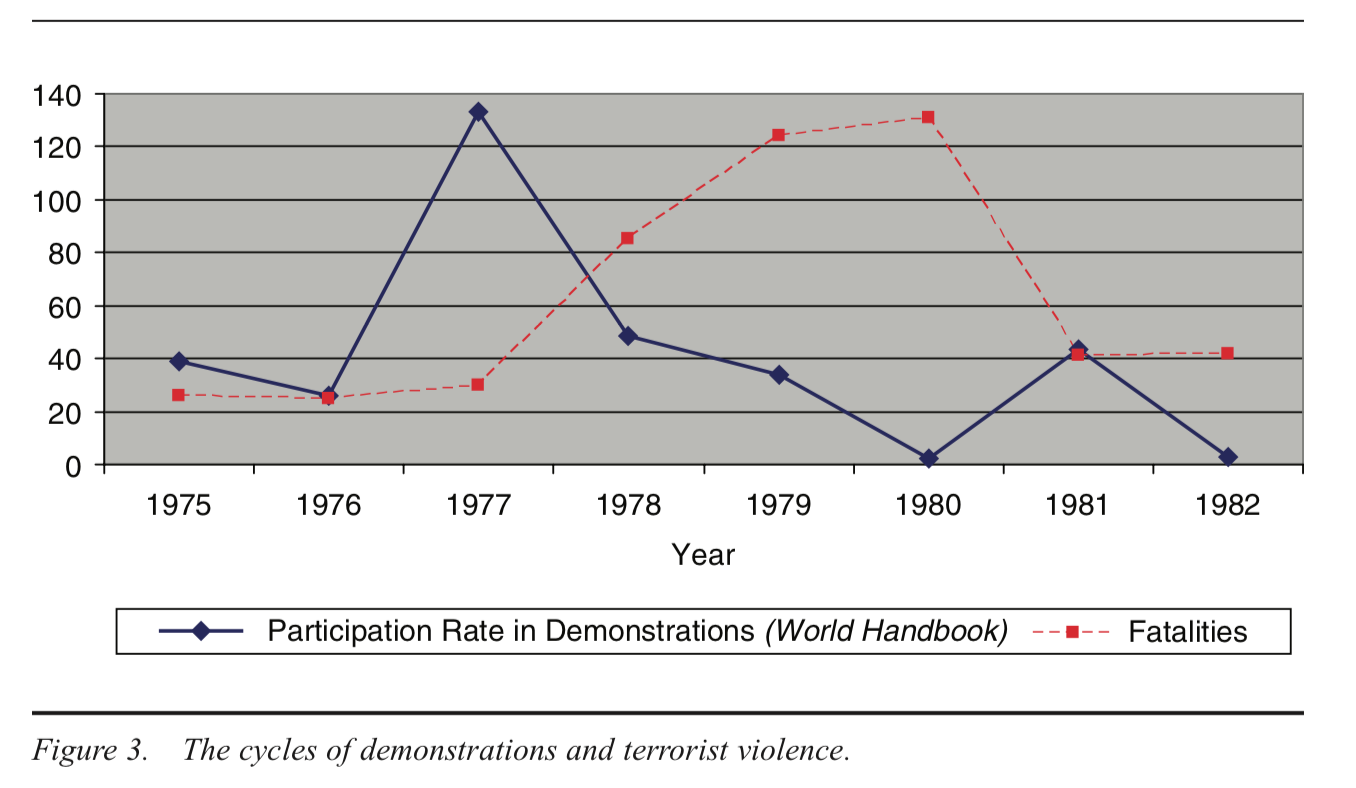
\includegraphics[width = 0.8\textwidth]{img/sanchez-cuenca-aguilar}

{\small Demonstrations and political violence during Spanish Transition}

\vspace{15pt}

{\tiny Ignacio Sánchez-Cuenca \& Paloma Aguilar (2009) Terrorist Violence and Popular Mobilization:\\The Case of the Spanish Transition to Democracy, \textit{Politics \& Society}, 37(3): 428--453.\\}

\end{frame}
% ----------------------------------------------------

% ----------------------------------------------------
\begin{frame}
\frametitle{Side gigs}
\centering

\visible<2>{\begin{minipage}{0.49\textwidth}\centering

\includegraphics[width = 0.8\textwidth]{img/nuklearra-ez}\\\vspace{10pt}

\includegraphics[width = 0.8\textwidth]{img/eta-mesa}
\end{minipage}}\hfill
\begin{minipage}{0.49\textwidth}\centering
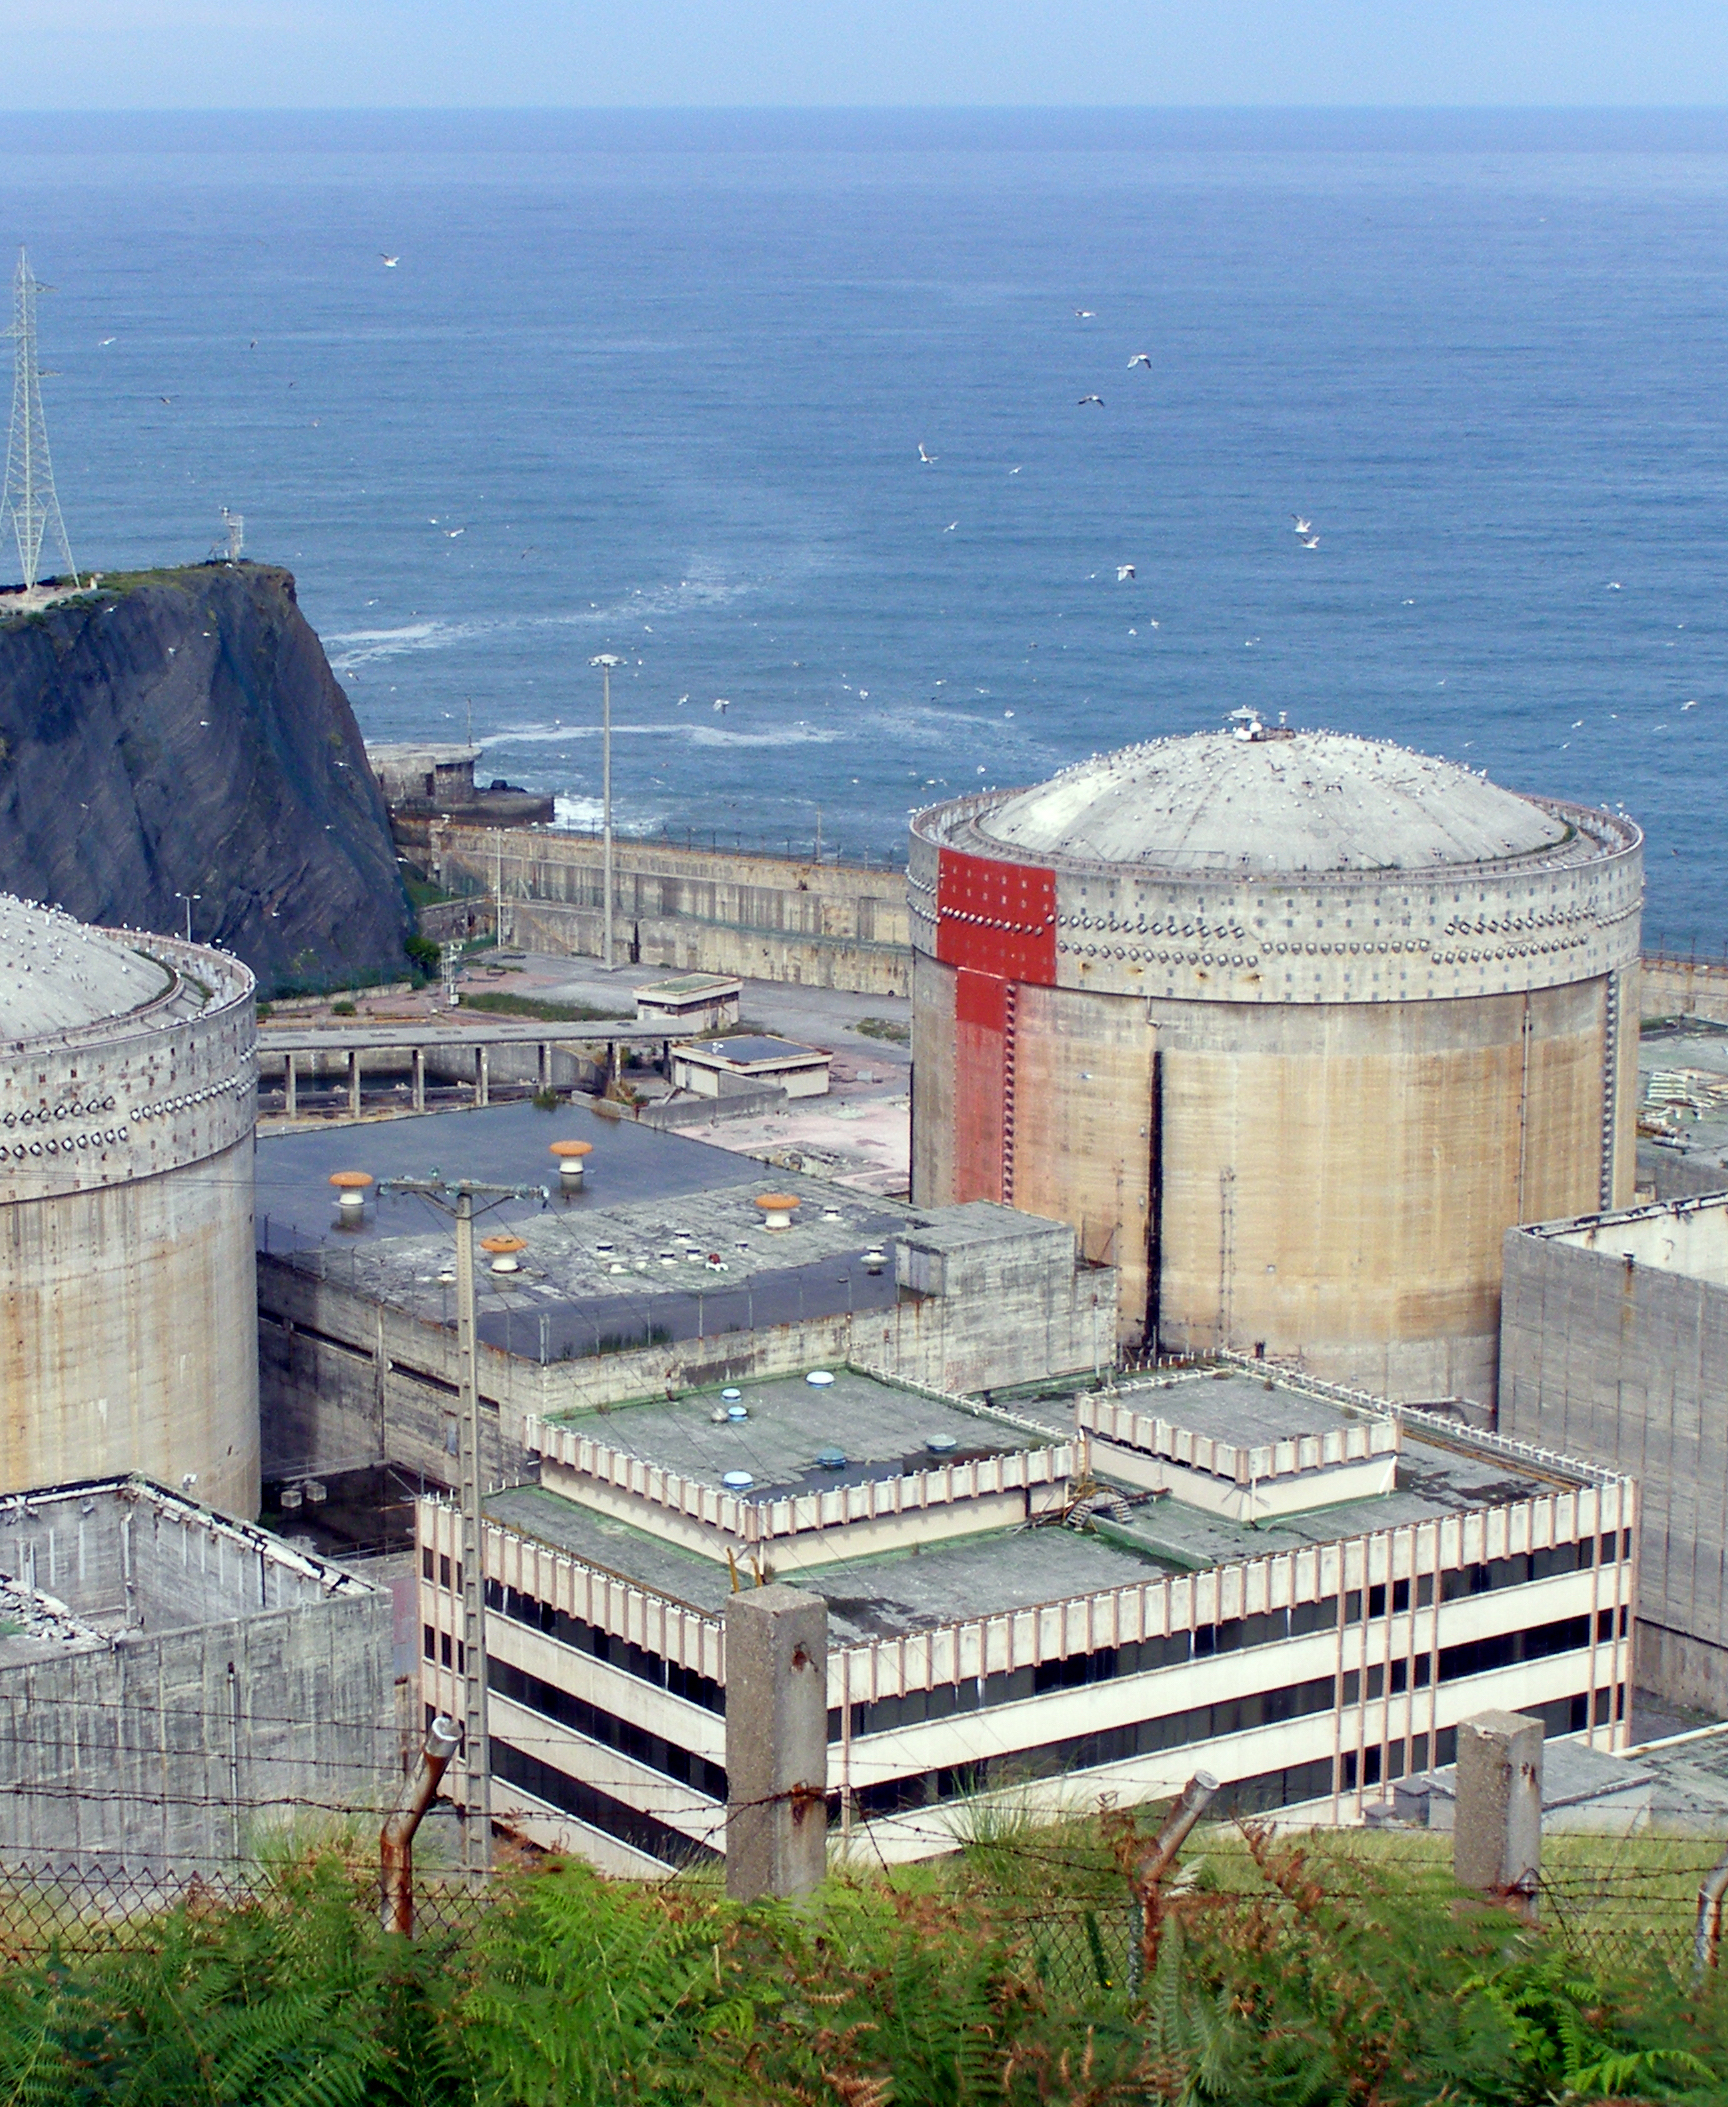
\includegraphics[width = \textwidth]{img/lemoiz}\\
{\small Lemoiz Nuclear Power Plant}
\end{minipage}

\end{frame}
% ----------------------------------------------------

% ----------------------------------------------------
\begin{frame}
\frametitle{Suicide bombing}
\centering

\begin{itemize}
  \item Suicide bombing, suicide attacks ...
  \item[] usually thought to be linked to terrorism
  \begin{itemize}
    \item<2-> Mostly, because of 9/11 and Islamist terrorist groups
    \item<3-> But not only: suicide attacks is a damage-maximizing method when there's no military capacity, so ideal for terrorist groups
  \end{itemize}
\end{itemize}

\end{frame}
% ----------------------------------------------------

% ----------------------------------------------------
\begin{frame}
\frametitle{Suicide bombing}
\centering

\begin{minipage}{0.49\textwidth}\centering
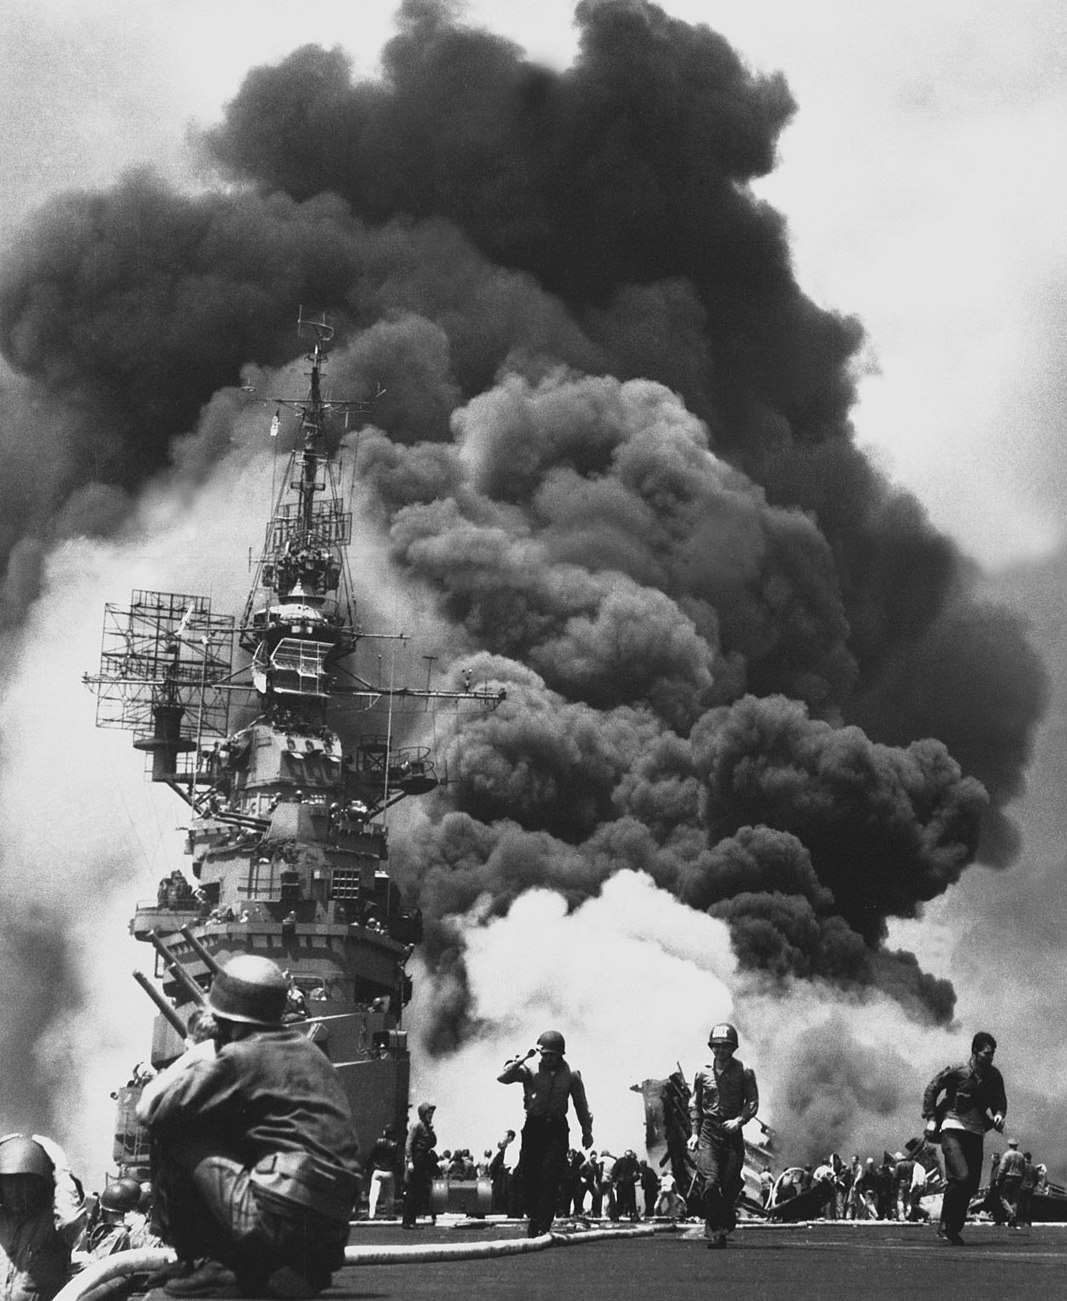
\includegraphics[width = 0.9\textwidth]{img/USS_Bunker_Hill_crop}\\{\footnotesize Attack on USS Bunker Hill, 1945}
\end{minipage}\hfill
\begin{minipage}{0.49\textwidth}\centering
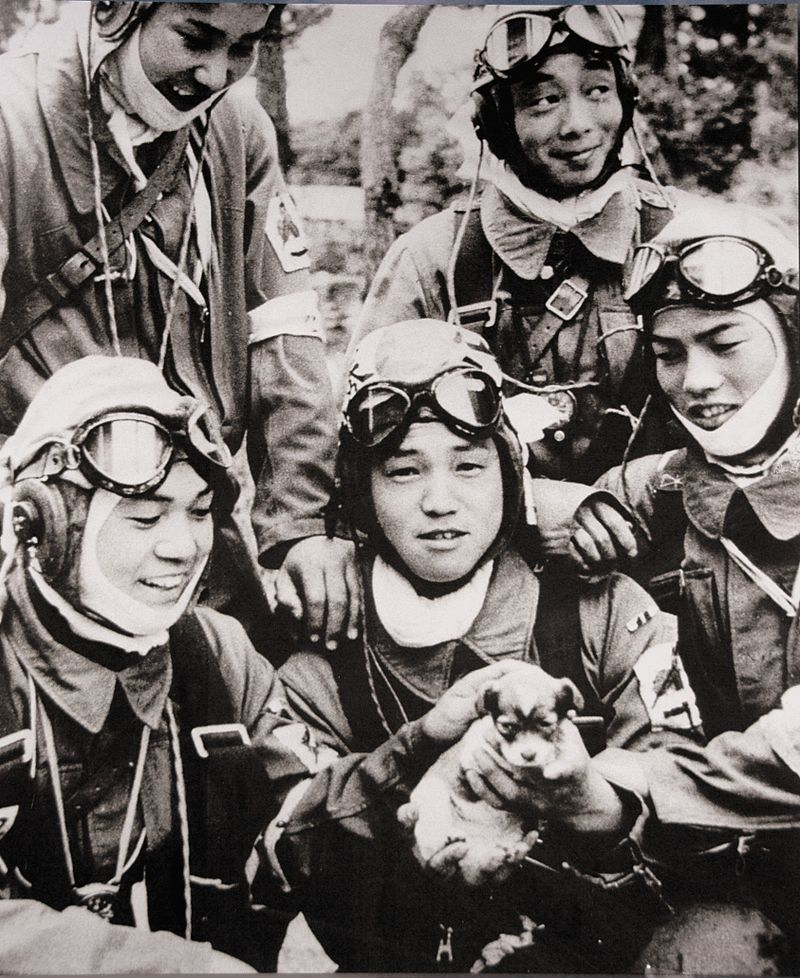
\includegraphics[width = 0.9\textwidth]{img/Kamikazes}
\end{minipage}

\end{frame}
% ----------------------------------------------------


% ----------------------------------------------------
\begin{frame}
\frametitle{Suicide bombing}
\centering

\begin{itemize}
  \item Modern suicide bombing after 1980s
  \item[]<2-> Lebanon (Hezbollah), Israel-Palestine (Hamas, Islamic Jihad), and Sri Lanka (LTTE), and became much more intense later in Iraq \& Afghanistan
\end{itemize}

\end{frame}
% ----------------------------------------------------

% ----------------------------------------------------
\imageframe{img/black_tigers}
% ----------------------------------------------------

% ----------------------------------------------------
\begin{frame}
\frametitle{Differences in suicide bombing use}
\centering

\begin{itemize}[<+->]
  \item Targeting civilians in Middle East
  \item Trained suicide bombers targeting high-rank military/civilian elites in Sri Lanka
\end{itemize}

\end{frame}
% ----------------------------------------------------

% ----------------------------------------------------
\imageframe{img/premadasa}
% ----------------------------------------------------

% ----------------------------------------------------
\begin{frame}
\frametitle{Trends in suicide bombing}
\centering

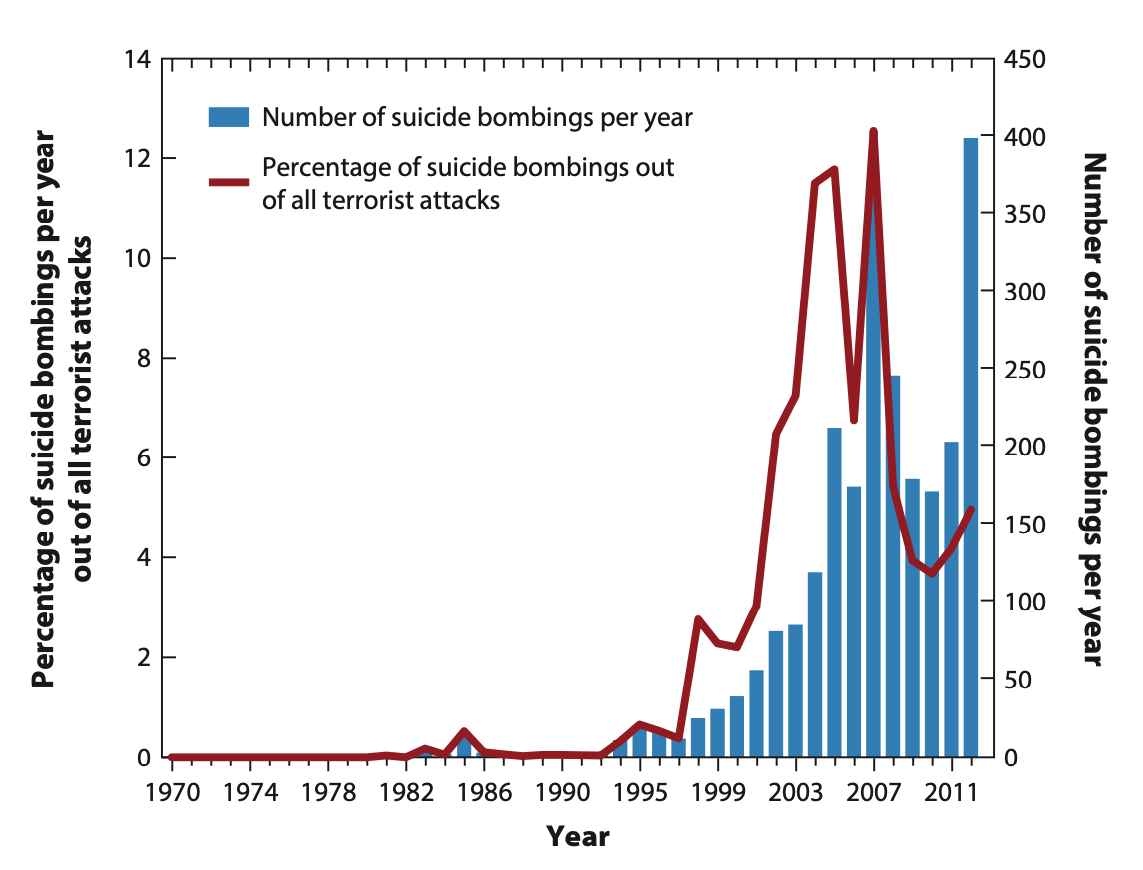
\includegraphics[width = 0.8\textwidth]{img/suicide_bombing_arps}

\end{frame}
% ----------------------------------------------------

% ----------------------------------------------------
\begin{frame}
\frametitle{Why does it happen?}
\centering

\begin{itemize}[<+->]
  \item We could think of factors at two levels
  \item[1.] Why do {\color{red}{individuals}} engage in suicide bombing?
  \begin{itemize}
    \item Obviously, not obvious why people kill themselves
  \end{itemize}
  \item[2.] Why do {\color{red}{groups}} employ it?
  \begin{itemize}
    \item Same for groups, why waste manpower?
  \end{itemize}
\end{itemize}

\end{frame}
% ----------------------------------------------------


% ----------------------------------------------------
\begin{frame}
\frametitle{Why does it happen?}
\centering

\begin{itemize}[<+->]
  \item[1.] {\color{red}{Individual motivations}}
  \begin{itemize}
    \item Early on, just irrationality?
    \item Variety of `justifications' proposed: intergenerational transfers, upholding group values, depression (not clear), grievances, indoctrination, etc
    \item Some use specific highly trained units (Black Tigers), while others recruit for one attack
    \item Is it poor people with nothing to lose?
    \item[] Not clear, actually wealthier than average by national standards
  \end{itemize}
\end{itemize}

\end{frame}
% ----------------------------------------------------

% ----------------------------------------------------
\begin{frame}
\frametitle{Suicide bombing}
\centering

\begin{itemize}[<+->]
  \item[2.] {\color{red}{Group tactical choice}}
  \begin{itemize}
    \item Religion: there's actually an association, but not clear why (`club goods', theology, ...?)
    \item Outbidding: groups competing, e.g. Hamas \& Islamic Jihad in Palestine
    \item Public opinion: more detached, more suicide bombing
    \item Organizations: newer, more `innovative' groups, larger groups that can afford losing members, ...?
  \end{itemize}
\end{itemize}

\end{frame}
% ----------------------------------------------------


\end{document}
